\chapter{Facial Feature Points Detection}
\label{sec:FFPD}

The second part of this report will focus on robust face feature detection for 2D images. As far as the method is concerned, again a regression forest similar to the one is used for the head pose estimation with a few variations will be built for purpose. In addition, a robust face detector \cite{facedetect} is also used as a prior step for landmark detection. Although, face detection is not exactly in the scope of this project, some of the necessary details for this algorithm will be mentioned in this chapter. Forest training will be discussed in \ref{sec:FT} and evaluation will be done in \ref{sec:FFeval}.

\clearpage
\section{Face Detection}
\label{sec:FD}
As a preliminary step for feature points detection, face detection is needed since feature points are local information which can only be found around the face area. Haar feature based classifiers are trained to form a such detector.

Firstly, for training images, both positive and negative images are needed. And referencing to sections \ref{sec:HLfeatures} and \ref{sec:integralimage}, rectangular features are calculated from sub windows extracted from each image. Since this pool of candidate features is very big, Adaboost is used to select the best features. \cite{facedetect}

For testing, the most area of an image is non face, we don't want apply every feature selected by Adaboost on every sub windows from test image. Therefore, Viola and Jones "introduce a method for constructing a cascade of classifiers to get good detection rate and decrease the computation time. The idea is to use classifier with less but efficient features to reject the majority of the sub-window before apply more complex classifiers". \cite{facedetect} The two features they used can be seen in Fig \ref{fig:strongclassifiers}. With the filtering procedure, time taken for processing each image is lower. The graphical description of such process can be seen from Fig \ref{fig:cascade}.

\begin{figure}
	\centering
	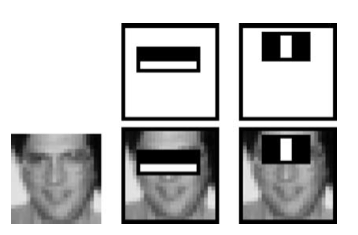
\includegraphics[width=0.8\linewidth]{facedetection.png}
	\caption[Two Efficient Selected by AdaBoost]{\label{fig:strongclassifiers}}  \textbf{"The two features are shown in the top row and then overlayed on a typical training face in the bottom row. The first feature measures the difference in intensity between the region of the eyes and a region across the upper cheeks. The feature capitalizes on the observation that the eye region is often darker than the cheeks. The second feature compares the intensities in the eye regions to the intensity across the bridge of the nose." \cite{facedetect}}
\end{figure}

\begin{figure}
	\centering
	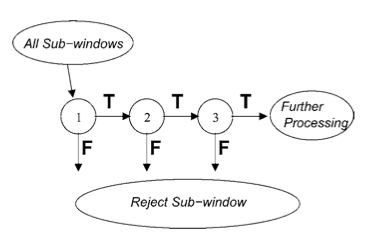
\includegraphics[width=0.8\linewidth]{cascade.png}
	\caption[Cascade Rejection]{\label{fig:cascade}}  \textbf{All sub windows are passed to the cascade of classifiers and in the early stages, the majority of sub windows will be rejected by the initial classifiers and fewer will be left for further processing  \cite{facedetect}}
\end{figure}

\newpage
\thispagestyle{plain}
\mbox{}

\section{Forest Training for Feature Detection}
\label{sec:FT}
Similar to the forest built in chapter \ref{sec:HPestimation}, trees are learned from randomly chosen subsets of all training images. a frontal face detector \cite{facedetect}(implemented by opencv as CascadeClassifier) is used to extract the face bounding box from the given image. Squared patches  $P = ( \alpha^{1},\alpha^{2} ,\theta )$ which are again marked positive and negative are randomly extracted within such bounding boxes and outside the box. Where $\alpha^{1}, \alpha^{2}$ are the image features used, which in this case is the grey values of the raw test images and the normalised grey values to compensate for illumination changes respectively as suggested by \cite{2dGFRF} and $\theta$ is the offset from each feature point to the centre of the patch. 

A pool of binary tests applied to patches at each non-leaf node is the same as did in section \ref{subsec:binarytest} by using equation \refeq{eq:binarytest} with different sub rectangular regions and thresholds. And Each node will split patches into two subsets, namely left and right as before.

Maximizing the information gain \refeq{eq:diffentropy} is required in order to find the best split in the pool. The measure of entropy $H{P}$ would be different from the one used in \ref{subsec:measureofentropy}. Since there are numbers of feature points to be located, $H_{r}(P)$ could be treat as the class uncertainty measure and it is defined as the following: \cite{2dGFRF}
\begin{equation}
\label{eq:classuncertainty}
H_{r}(P) = -\sum\limits_{n=1}^N \frac{\sum\nolimits_{i}p(c_{n}|P_i)}{|P|}log(\frac{\sum\nolimits_{i}p(c_{n}|P_i)}{|P|})
\end{equation}

\begin{equation}
\label{eq:classaffiliation}
p(c_{n}|P_i) \propto exp(- \frac{|d_{i}^{n}|}{\lambda})
\end{equation}

Where $p(c_{n}|P_i)$ is the probability of a given patch ${P_i}$ belongs to the feature point n, which is based on the distance between the patch centre and each of the landmark position. \cite{2dGFRF} And is proportional to $exp(- \frac{|d_{i}^{n}|}{\lambda})$.  Since we still need to classify each patch during testing at the leaf nodes, a measure of the class uncertainty is required. The measure $H_{c}(P)$as described in equation \refeq{eq:cumeasure} is used here. Same as the head pose estimation, $H_{c}(P)$ and $H_{r}(P)$ are combined by a weighted sum as in equation \refeq{eq:okada}. The best test parameters found will be store for each non leaf node.

The objective of forest in chapter \ref{sec:HPestimation} is to predict the location of the nose tip, whereas in this case, there are dozens of landmark locations to infer. Therefore at leaf nodes, the mean and trace of covariance matrices of the offsets to each feature points have to be store.

\newpage
\thispagestyle{plain}
\mbox{}

\section{Evaluation}
\label{sec:FFeval}
The dataset used for this experiment is FaceWarehouse \cite{facewarehouse}. There are 150+ test subjects and each of which has 20 different images taken with various facial expressions. 74 facial landmarks are annotated with each image. 17 of the facial landmarks such as eye brows, nose, eyes, and mouth were chosen for the purpose of this experiment as shown in Fig \ref{fig:expimage}. Image resolution is 640 $\times$ 480. And the faces in this dataset are all frontal faces.

During training, a frontal face detector \cite{facedetect}(implemented by opencv as CascadeClassifier) is used to extract the face from the given image. (shown in Fig \ref{fig:boundingbox}). Once the face bounding box is obtained, random patches with size of 80 $\times$ 80 (same size as used for head pose estimation) are extracted according to the bounding box. Number of patches sampled per training image is 80, one quarter of which are negative patches sampled outside the bounding box and the rest is positive patches. The $\lambda$ in equation \refeq{eq:classaffiliation} is set to 0.125 for this experiment as suggested by \cite{2dGFRF}. 

During testing, for each input image, face is initially extracted to obtain the bounding box ,in which test patches are densely sampled. Each patch is then passed to the trees in the forest where binary tests are performed at each non leaf node with the parameters stored during training. Once the patch reaches the leaf node, the two necessary conditions for a patch to cast a vote for the location of each feature point are as follows. Firstly, the class probability at that leaf node has to be 1 since with the distortion of negative patches, the distribution stored at leaf node is less informative. Secondly, for every leaf node, trace of covariance matrices for each feature point are stored during training, if such trace exceed certain threshold, the patch will not be allowed to cast a vote for the corresponding feature location. The remaining candidate votes are then filtered by mean shift to remove outliers in order to produce the final estimate.

The successful detection for a feature point is determined by whether the estimated point is within a certain region of the actual point. Such region is define by a circle centred at the ground truth point with a radius of 8 pixels as shown in figure \ref{fig:successregion}. Examples of false detection and true detection are shown in figures \ref{fig:fail} and \ref{fig:success}.


\begin{figure}
	\centering
	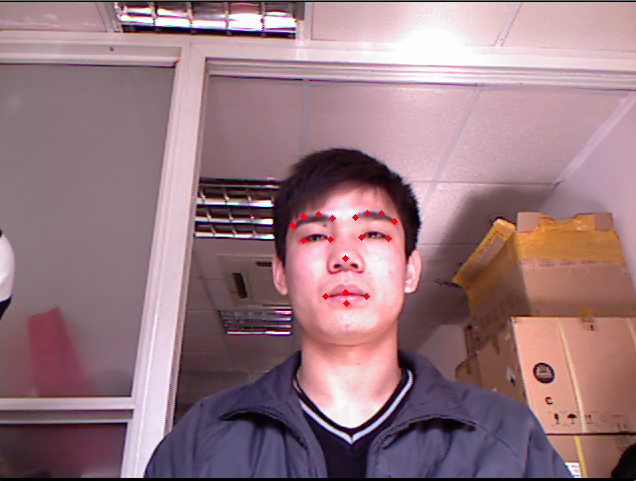
\includegraphics[width=0.8\linewidth]{Screenshot3.png}
	\caption[Landmarks chosen for experiment]{\label{fig:expimage}}  \textbf{Example of an image used for feature points detection, landmarks are marked in red }
\end{figure}

\begin{figure}
	\centering
	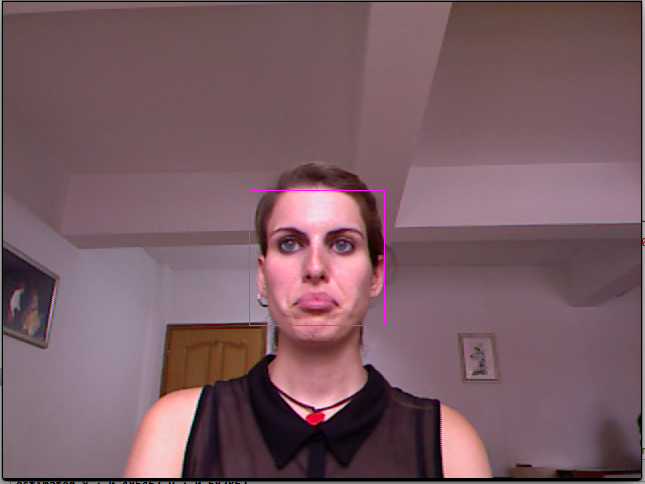
\includegraphics[width=0.8\linewidth]{boundingbox.png}
	\caption[Face detection]{\label{fig:boundingbox}}  \textbf{The region inside the purple bounding box is extracted face }
\end{figure}

\begin{figure}
	\centering
	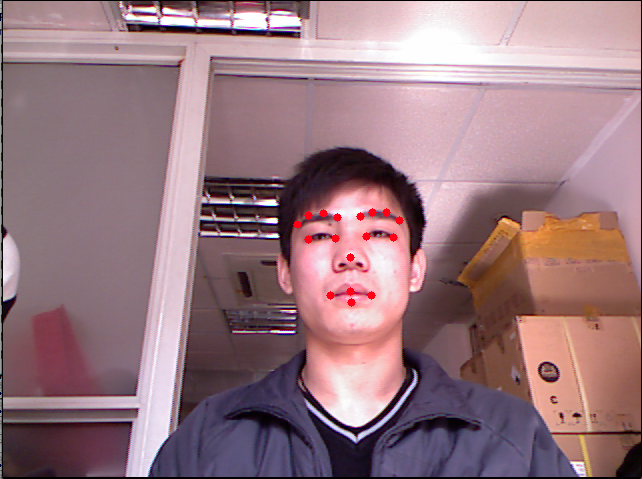
\includegraphics[width=0.8\linewidth]{Screenshot6.png}
	\caption[Landmarks Success Region]{\label{fig:successregion}}  \textbf{The red circles are the error tolerance region for each feature point}
\end{figure}

\begin{figure}
	\centering
	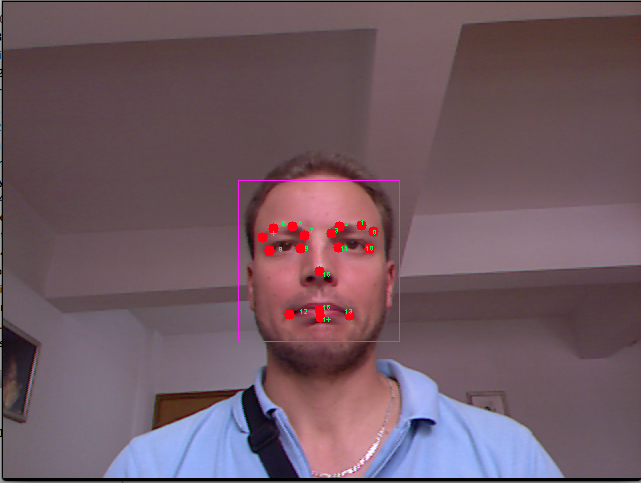
\includegraphics[width=0.8\linewidth]{fail.png}
	\caption[False Detection]{\label{fig:fail}}  \textbf{Example for false detection for some feature points such as points near right eye brow}
\end{figure}

\begin{figure}
	\centering
	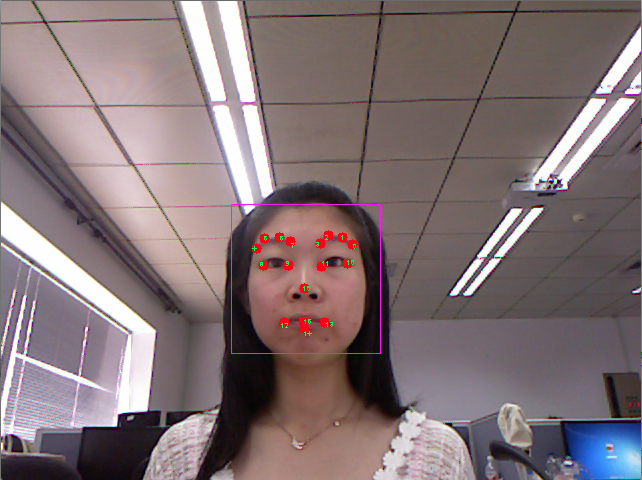
\includegraphics[width=0.8\linewidth]{success.png}
	\caption[Success Detection]{\label{fig:success}}  \textbf{Majority of the features are detected within the margin of error}
\end{figure}

For this experiment, 10 trees are trained and as the number of tree loaded, the accuracy improves as expected as can be seen from the plots \ref{fig:eyebrows},\ref{fig:eyes} and \ref{fig:noseandmouth}. Overall, success rate of feature points around eyes and nose area is higher than the detection rate around mouth. The reason for such low performance around mouth area might due to the huge deformations. When patches are sampled at a density of 5 stride, the overall accuracy is about  3\% higher than when sampled at 10 stride. 

\begin{figure}
        \centering
	 \begin{subfigure}[b]{0.5\textwidth}
                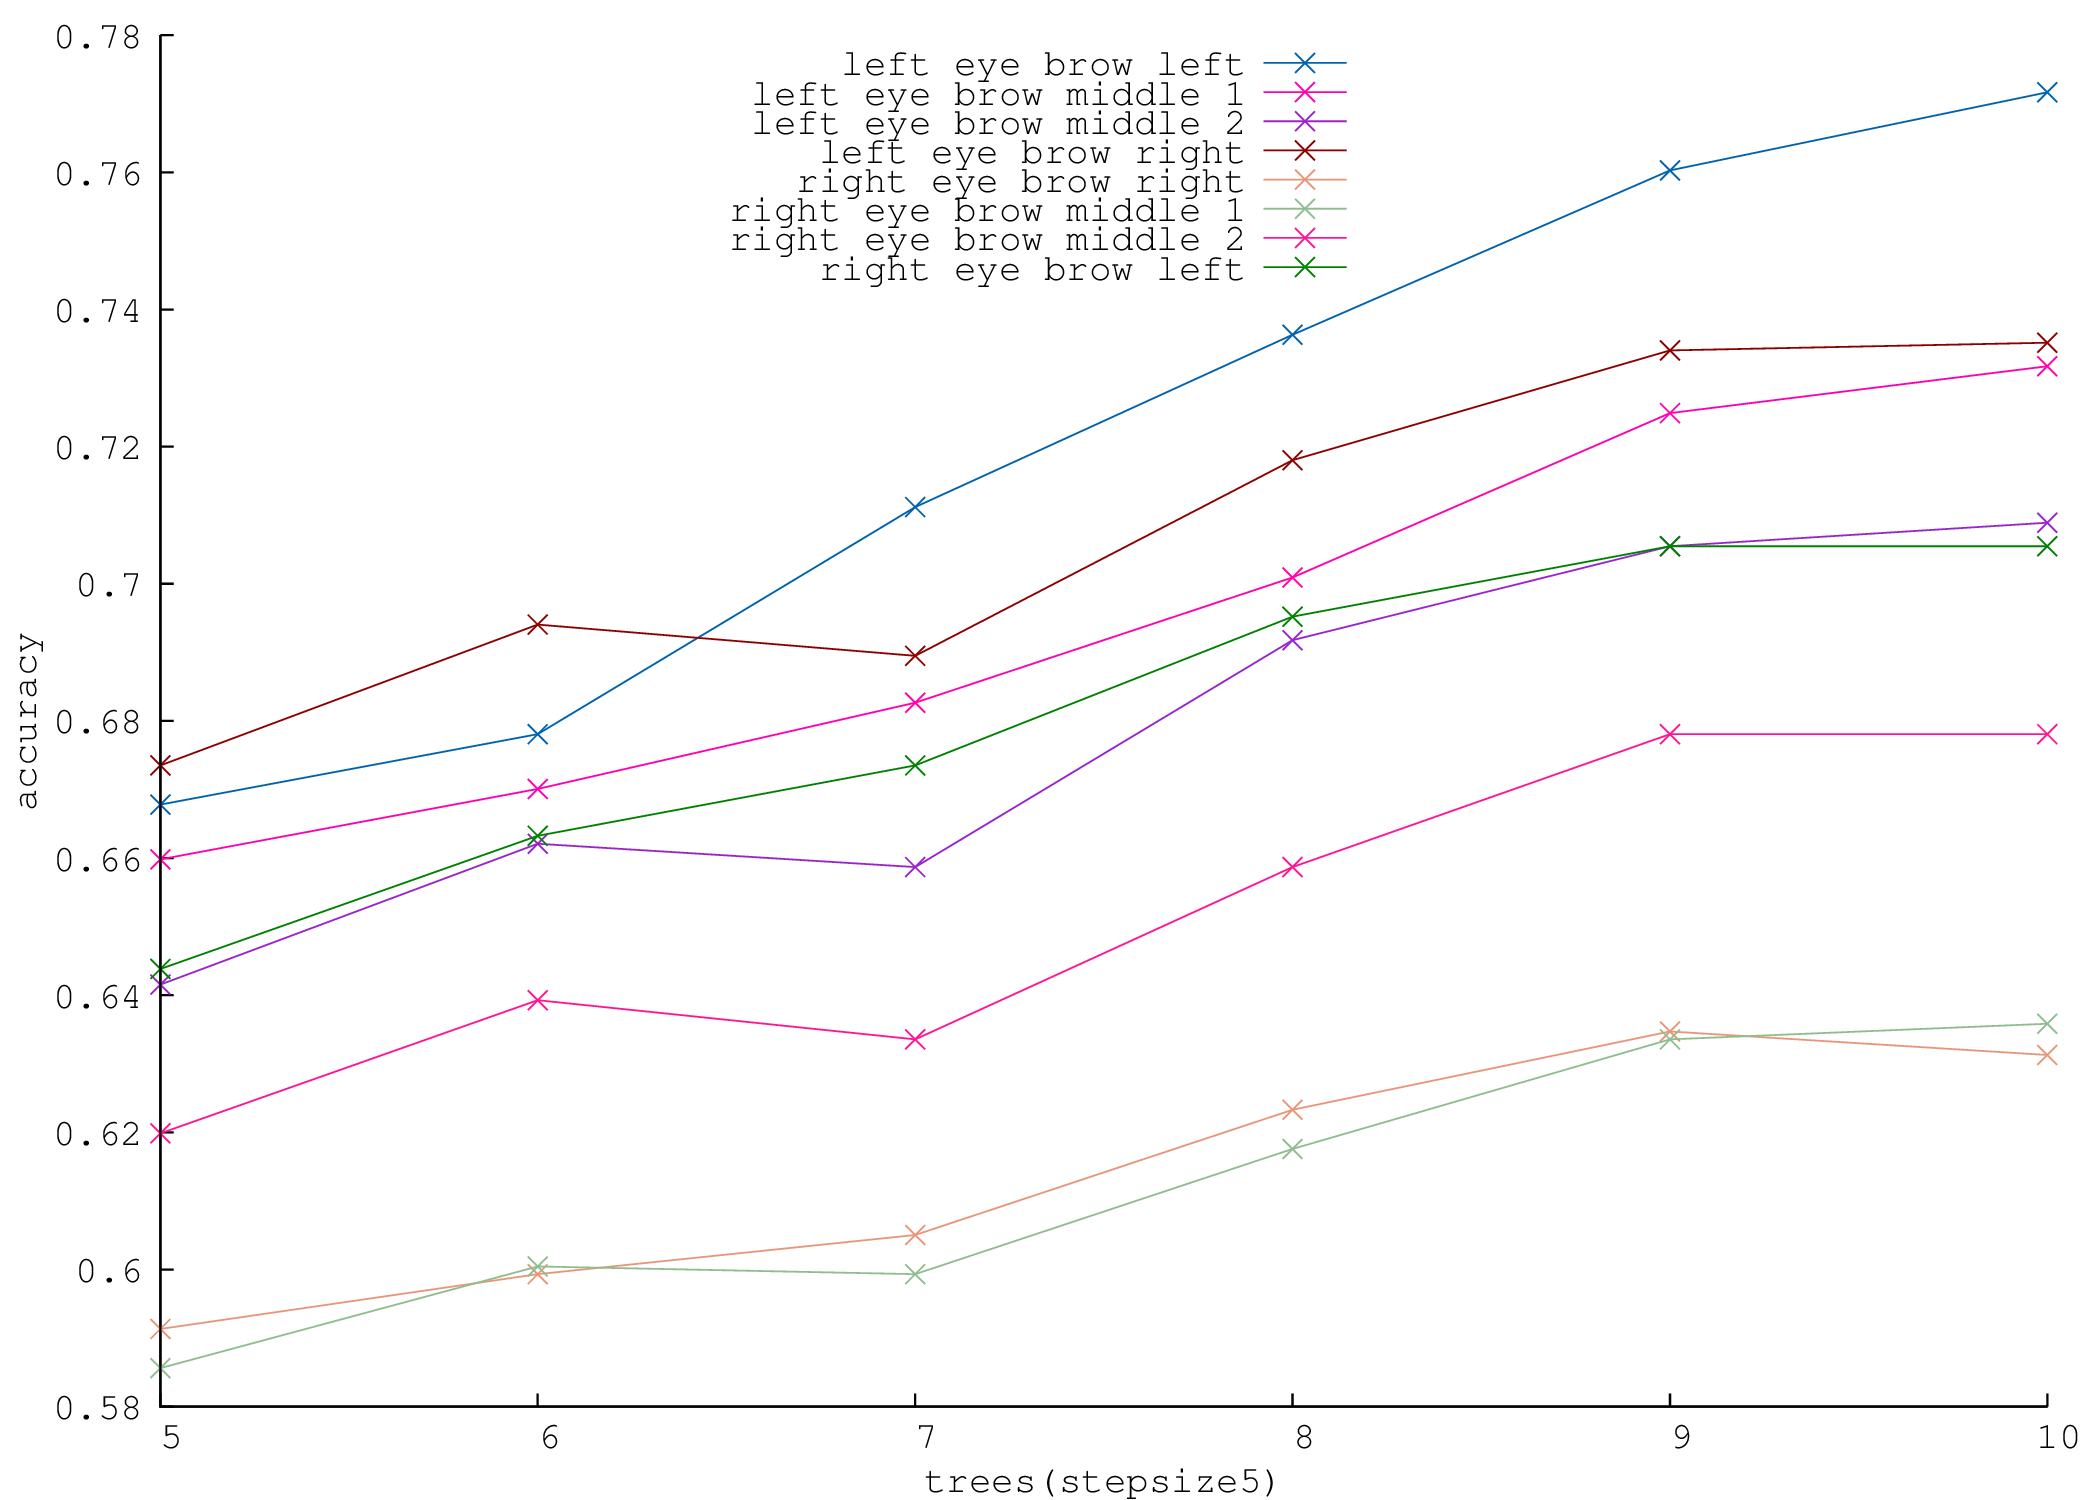
\includegraphics[width=\textwidth]{eyebrowaccuracyvstrees2dss5.png}
                \caption{stride 5}
                \label{fig:eyebrowstride5}
        \end{subfigure}%
        \begin{subfigure}[b]{0.5\textwidth}
                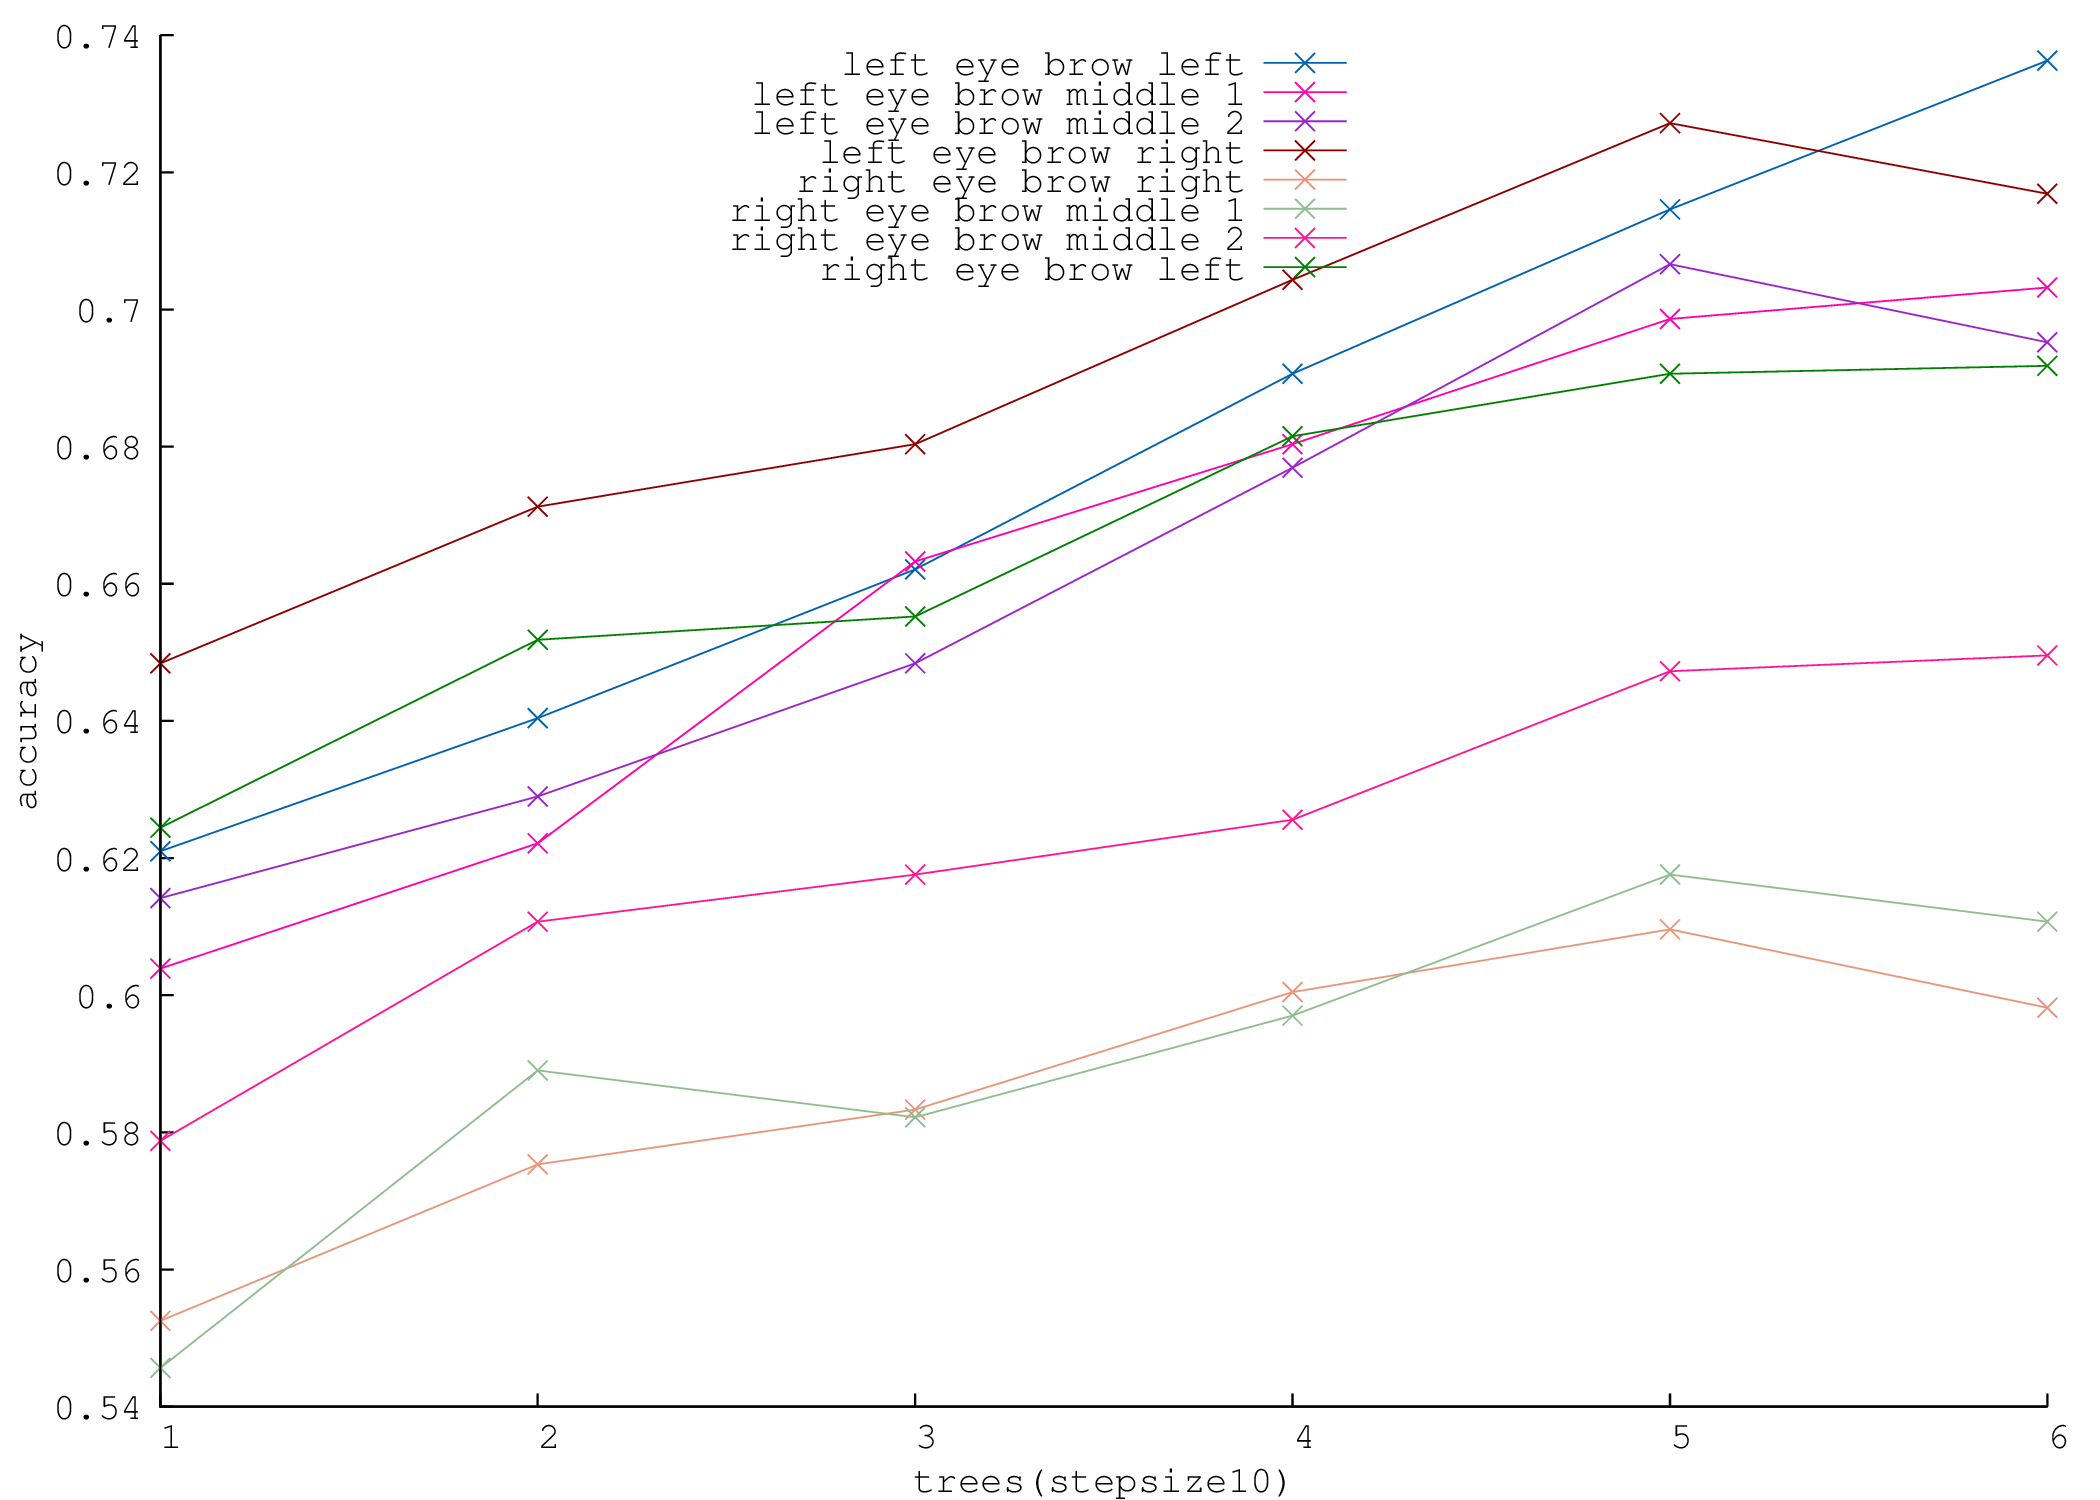
\includegraphics[width=\textwidth]{eyebrowaccuracyvstrees2dss10.png}
                \caption{stride 10}
                \label{fig:eyebrowstride10}
        \end{subfigure}%
        \caption{Eye brows accuracy vs number of trees}\label{fig:eyebrows}
\end{figure}

\begin{figure}
        \centering
	 \begin{subfigure}[b]{0.5\textwidth}
                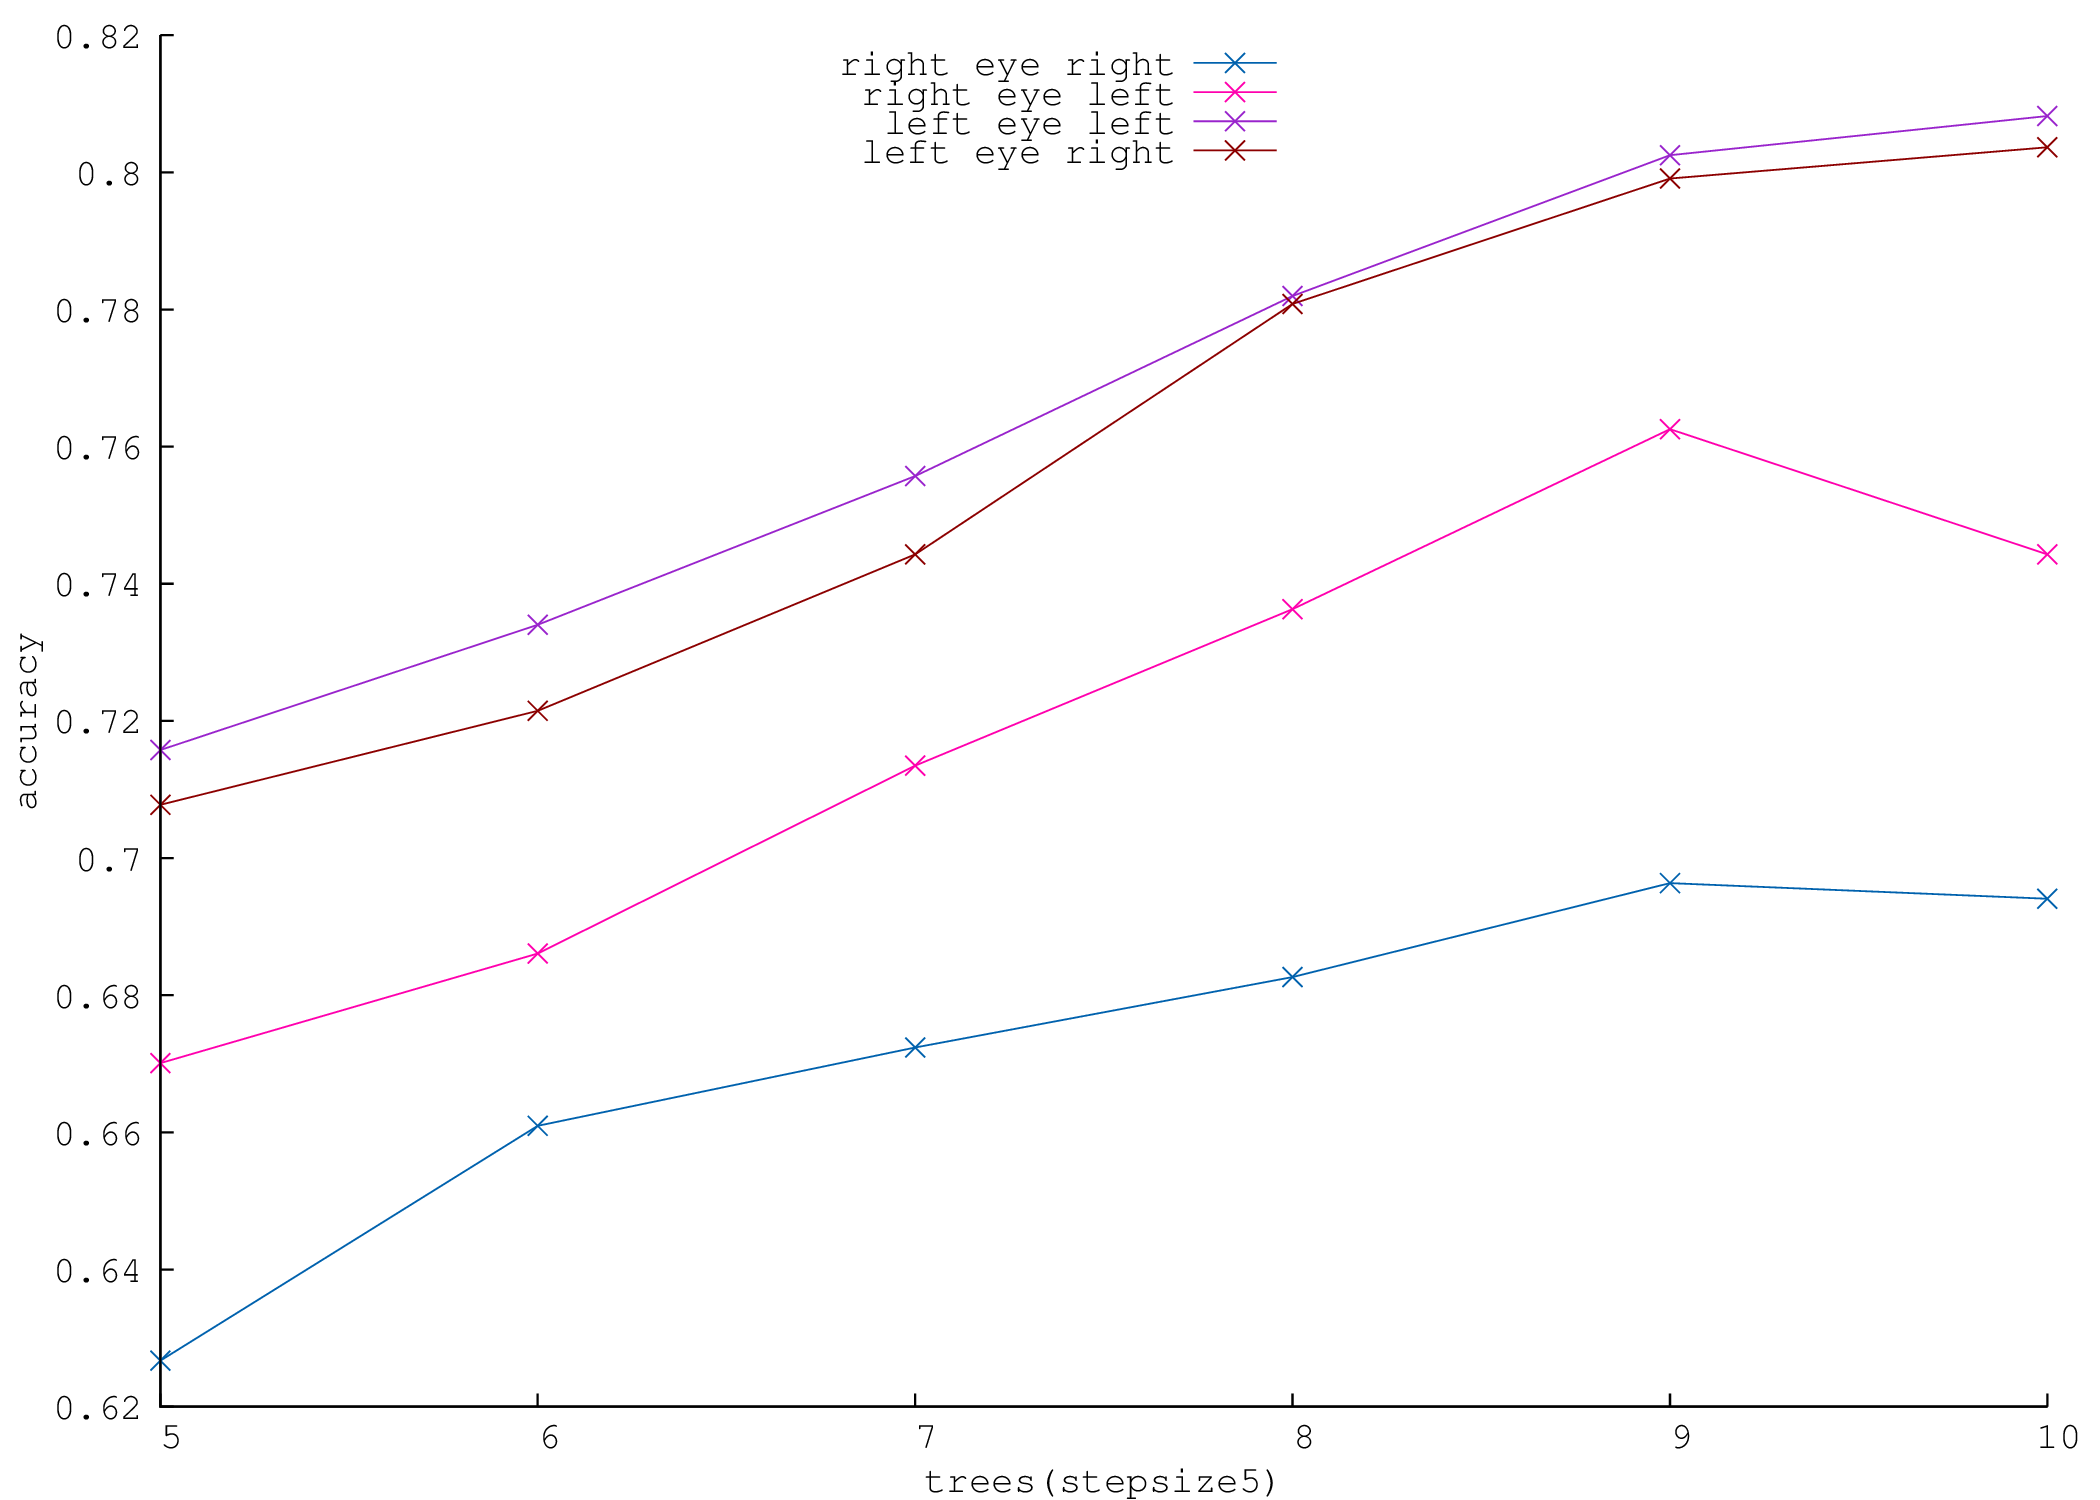
\includegraphics[width=\textwidth]{eyesaccuracyvstrees2dss5.png}
                \caption{stride 5}
                \label{fig:eyesstride5}
        \end{subfigure}%
        \begin{subfigure}[b]{0.5\textwidth}
                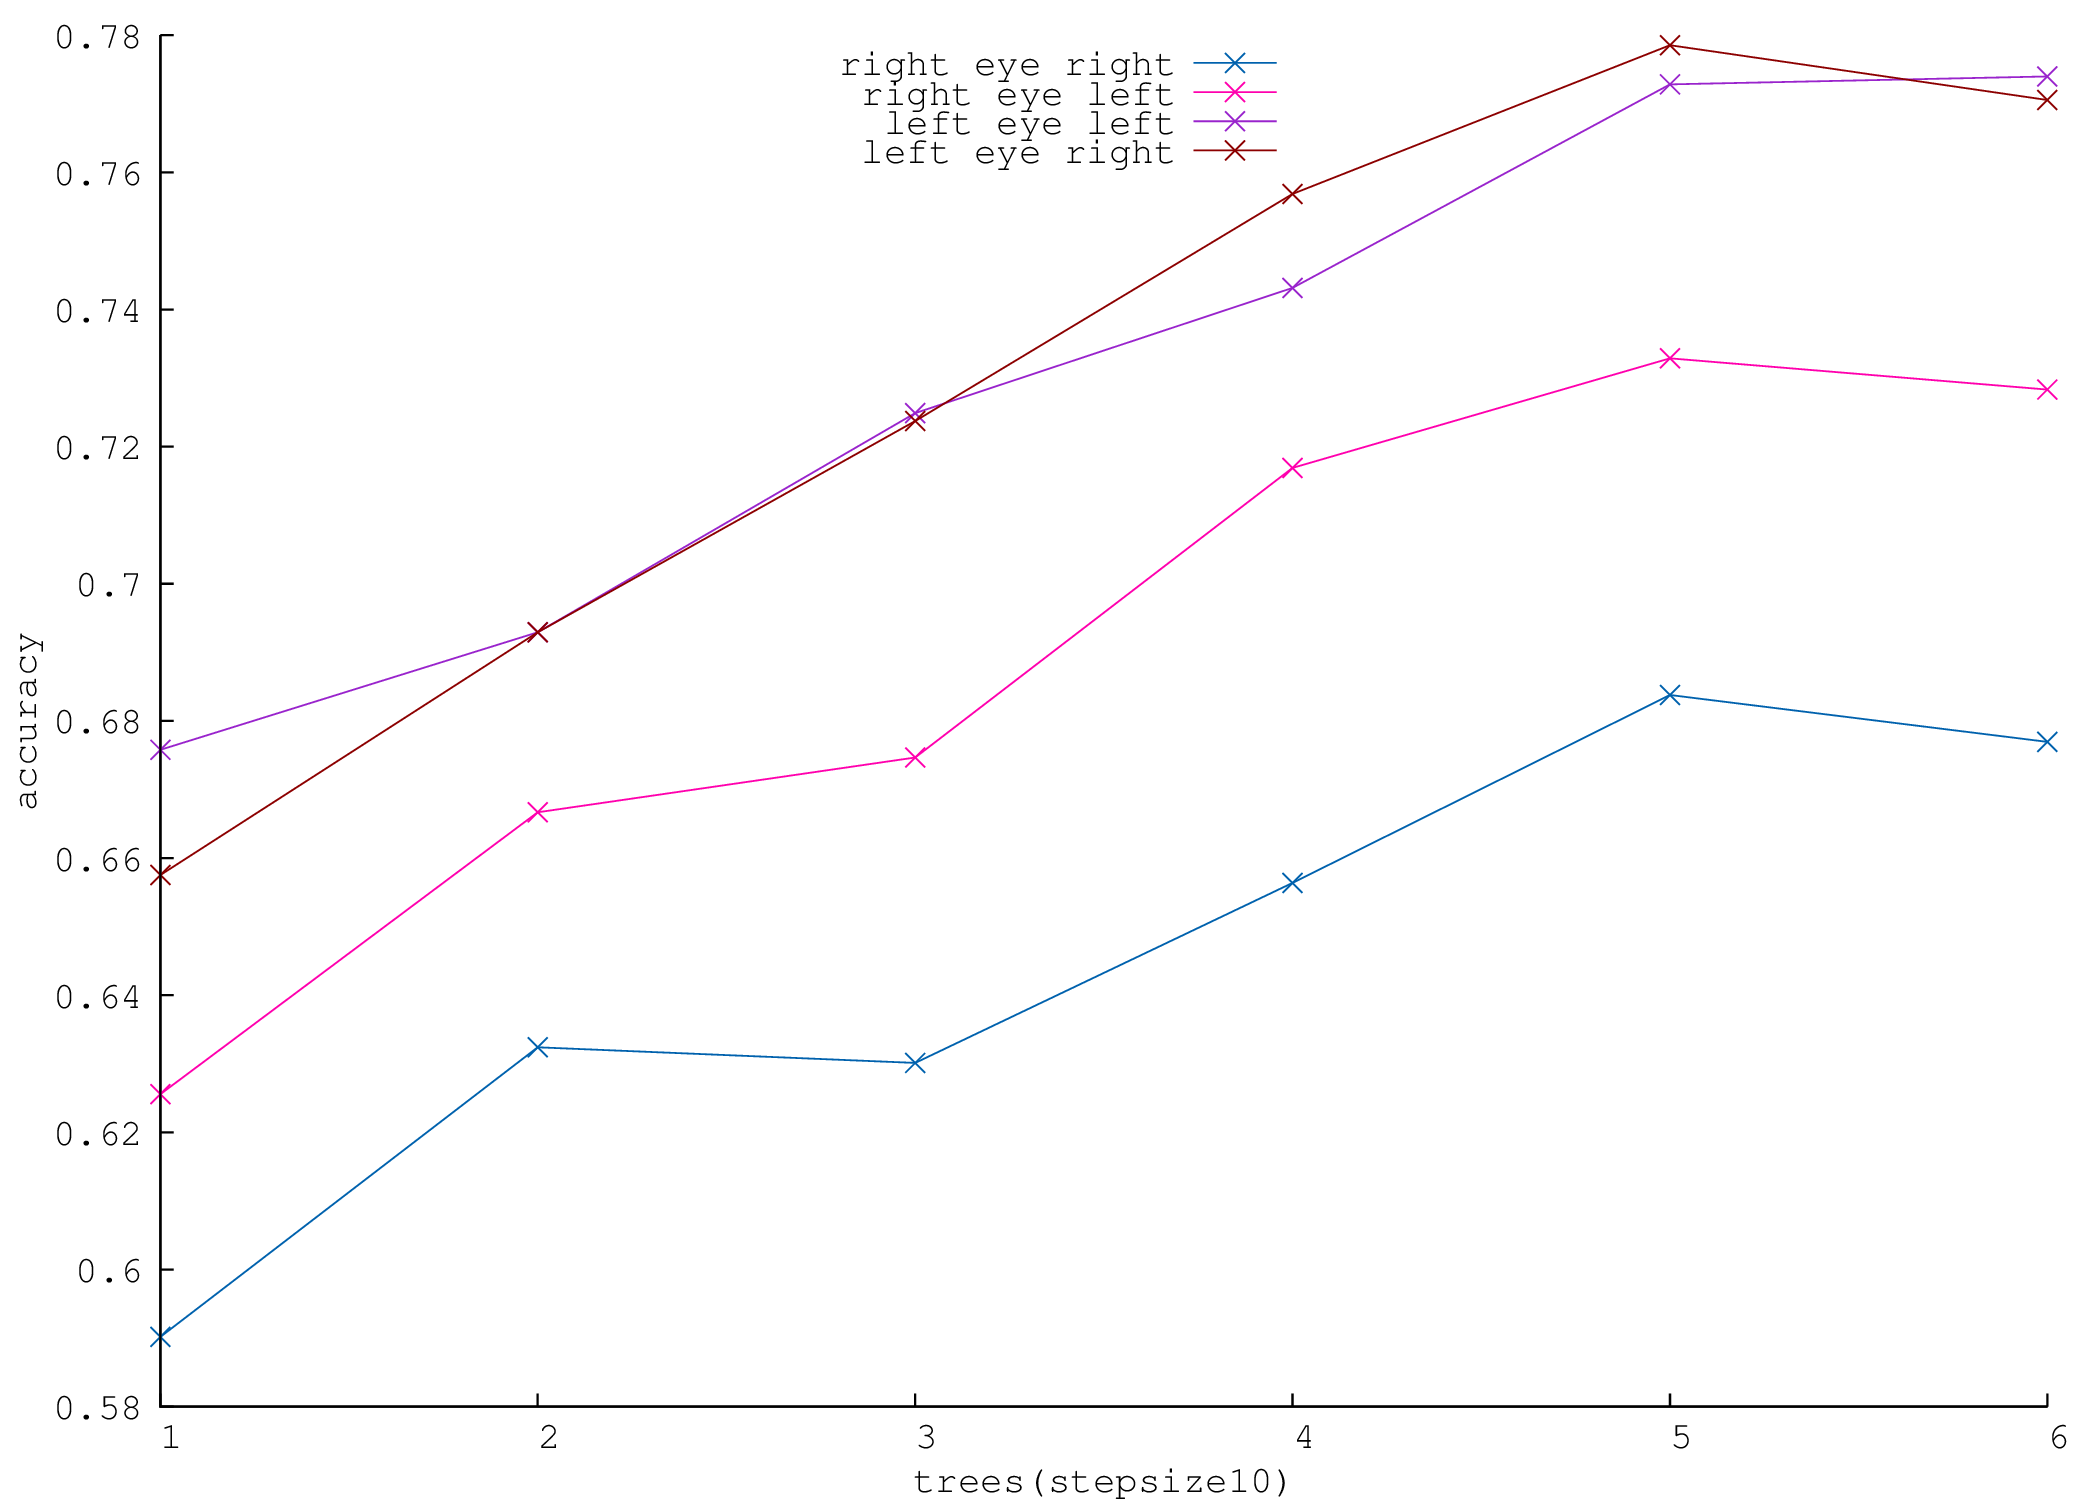
\includegraphics[width=\textwidth]{eyesaccuracyvstrees2dss10.png}
                \caption{stride 10}
                \label{fig:eyestride5}
        \end{subfigure}%
        \caption{Eyes accuracy vs number of trees}\label{fig:eyes}
\end{figure}

\begin{figure}
        \centering
	 \begin{subfigure}[b]{0.5\textwidth}
                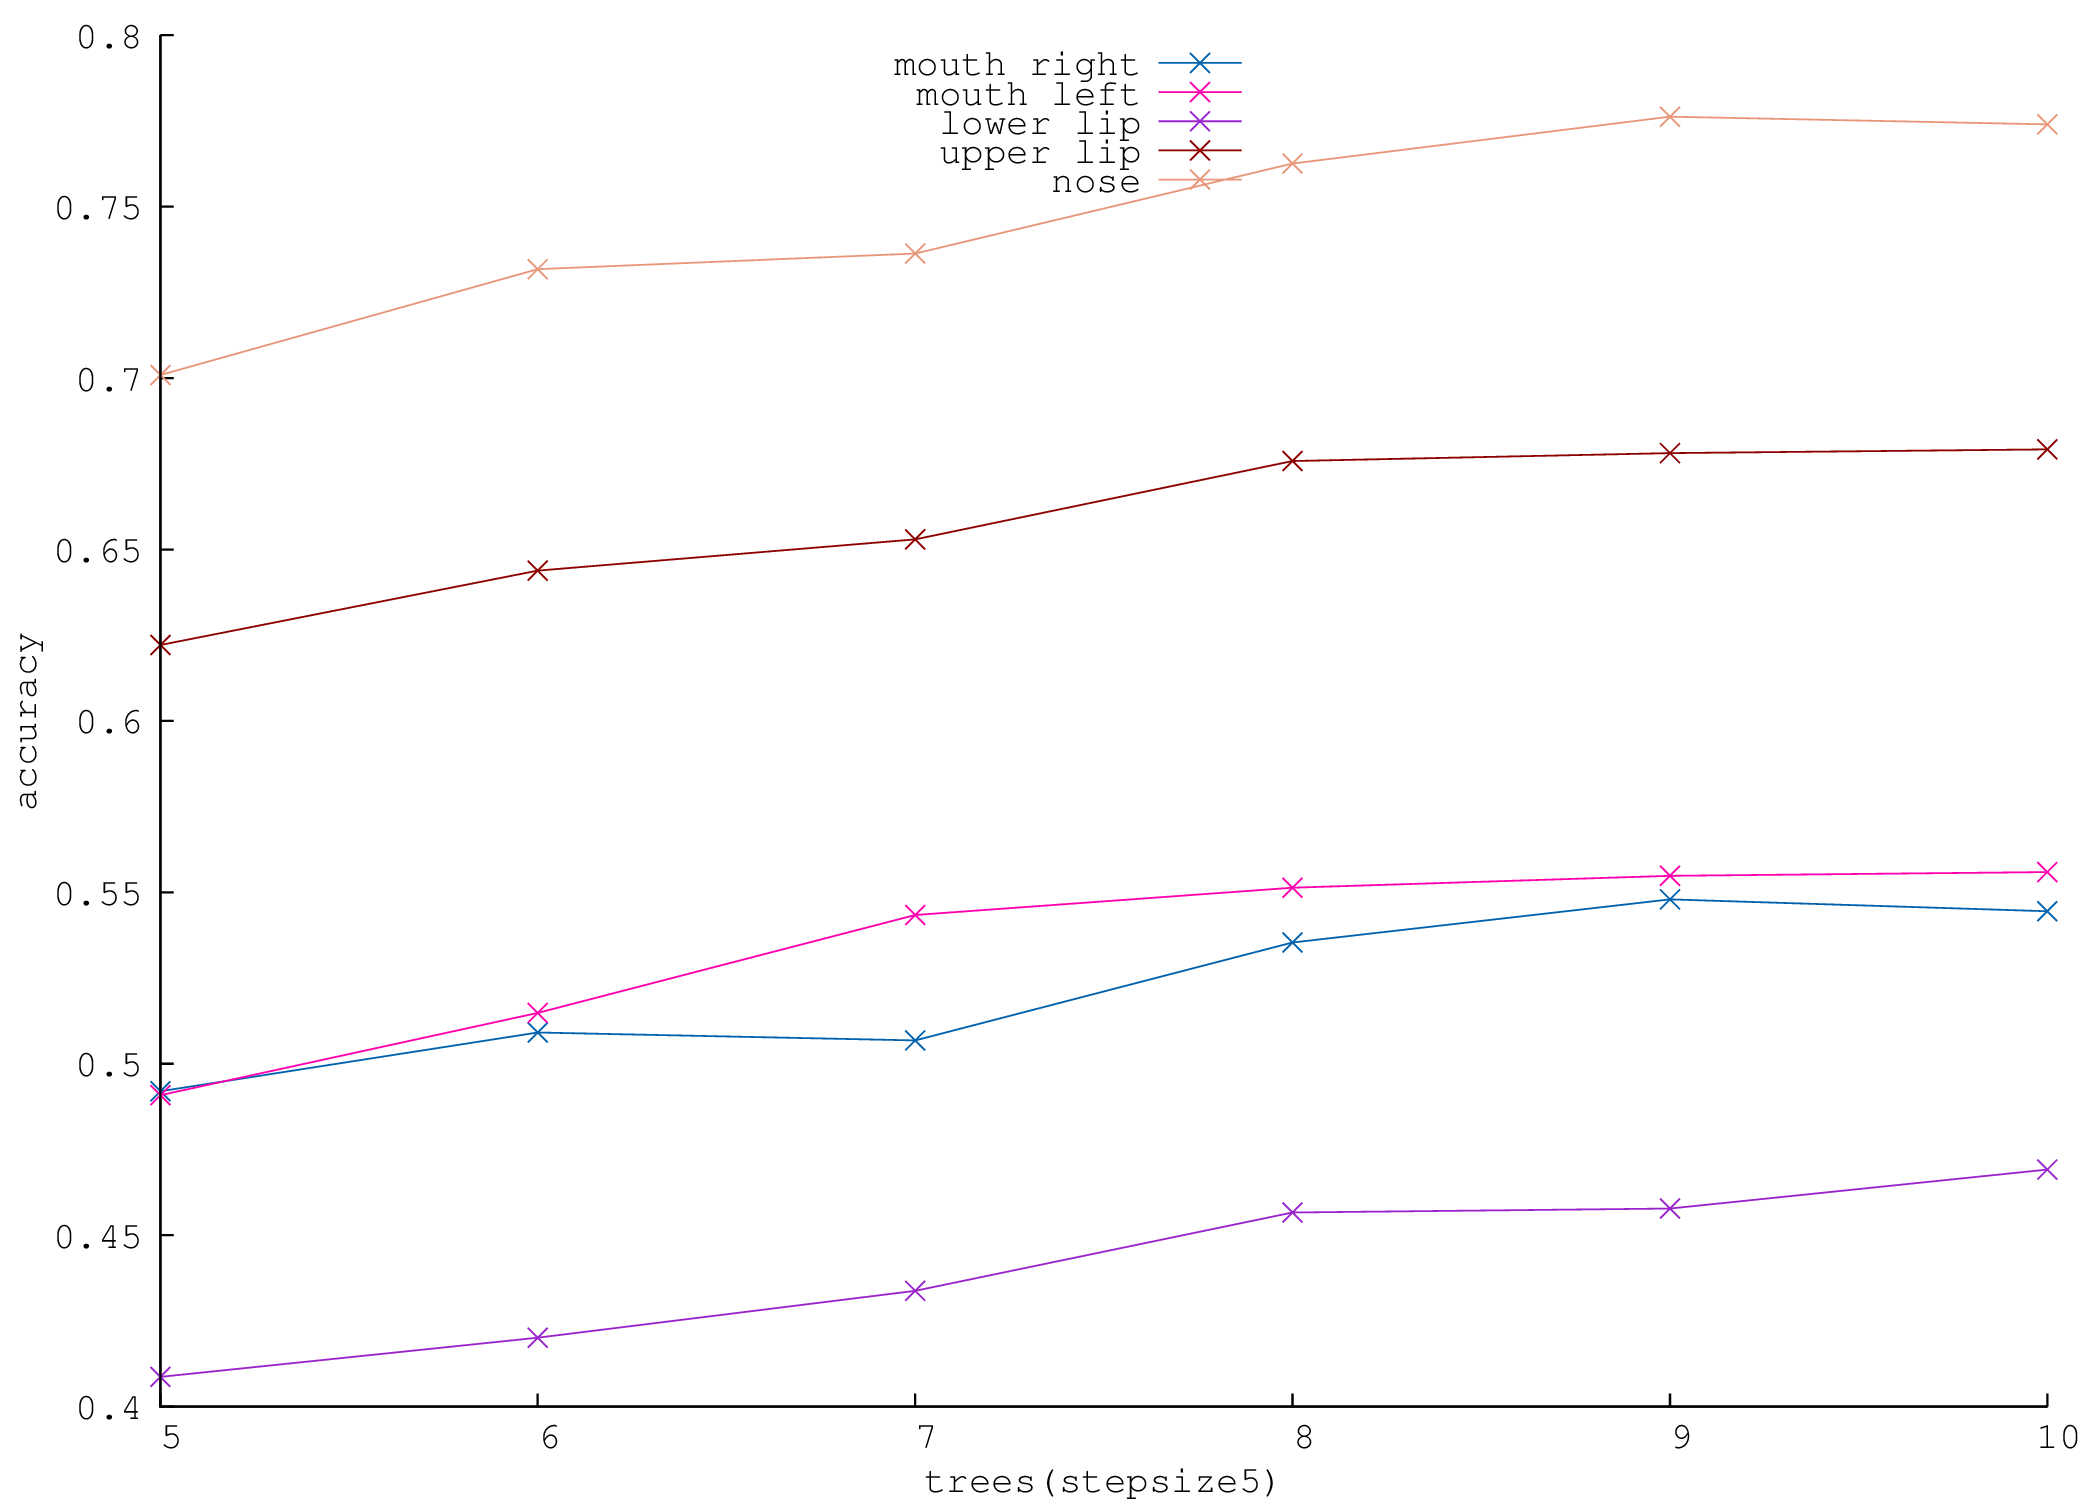
\includegraphics[width=\textwidth]{nosemouthaccuracyvstrees2dss5.png}
                \caption{stride 5}
                \label{fig:eyesstride5}
        \end{subfigure}%
        \begin{subfigure}[b]{0.5\textwidth}
                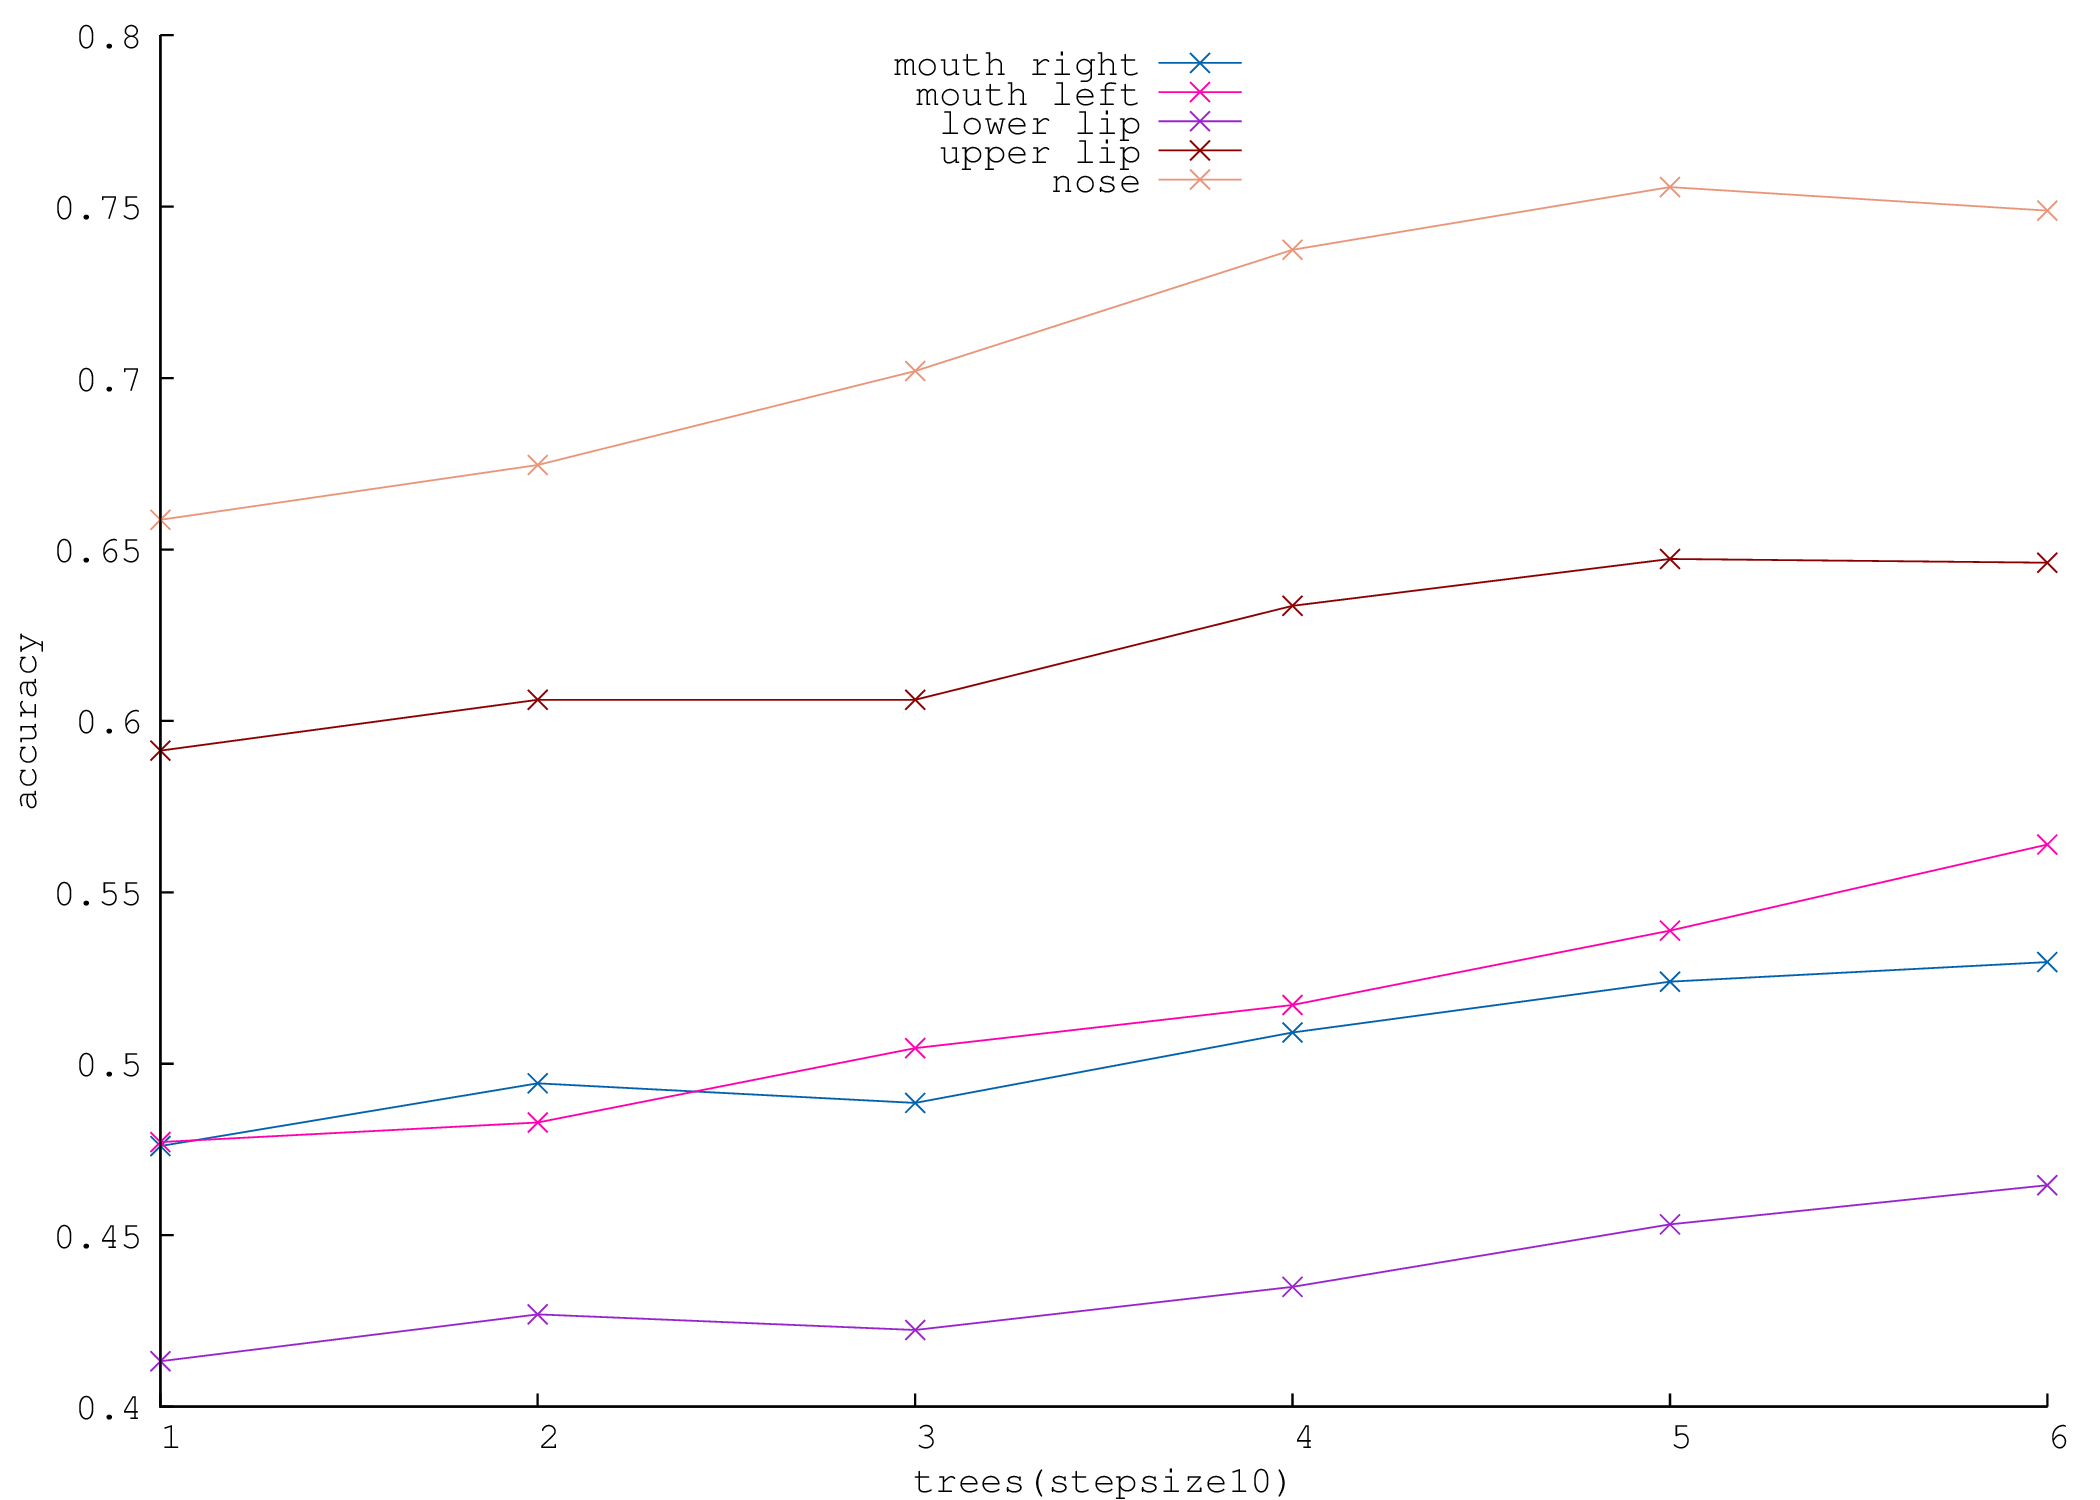
\includegraphics[width=\textwidth]{nosemouthaccuracyvstrees2dss10.png}
                \caption{stride 10}
                \label{fig:eyestride5}
        \end{subfigure}%
        \caption{Nose and mouth accuracy vs number of trees}\label{fig:noseandmouth}
\end{figure}

In addition, speed is also an important parameter in performance and the time taken to process each image is proportional number of patches sampled. Figure \ref{fig:time} shows the relationship between the average time taken to process each image after it has been loaded into memory and the number of trees load. When sampling at a density of 5 stride and 10 trees are loaded, the time taken is approximately 0.1 seconds. In other words, at this sampling density, the system can handle 10 frames per second. However, the computation time decreases to only 0.04 seconds (25 frames per second) when patches are sampled at stride 10 which is a 3 \% drop in accuracy on average.


\begin{figure}
	\centering
	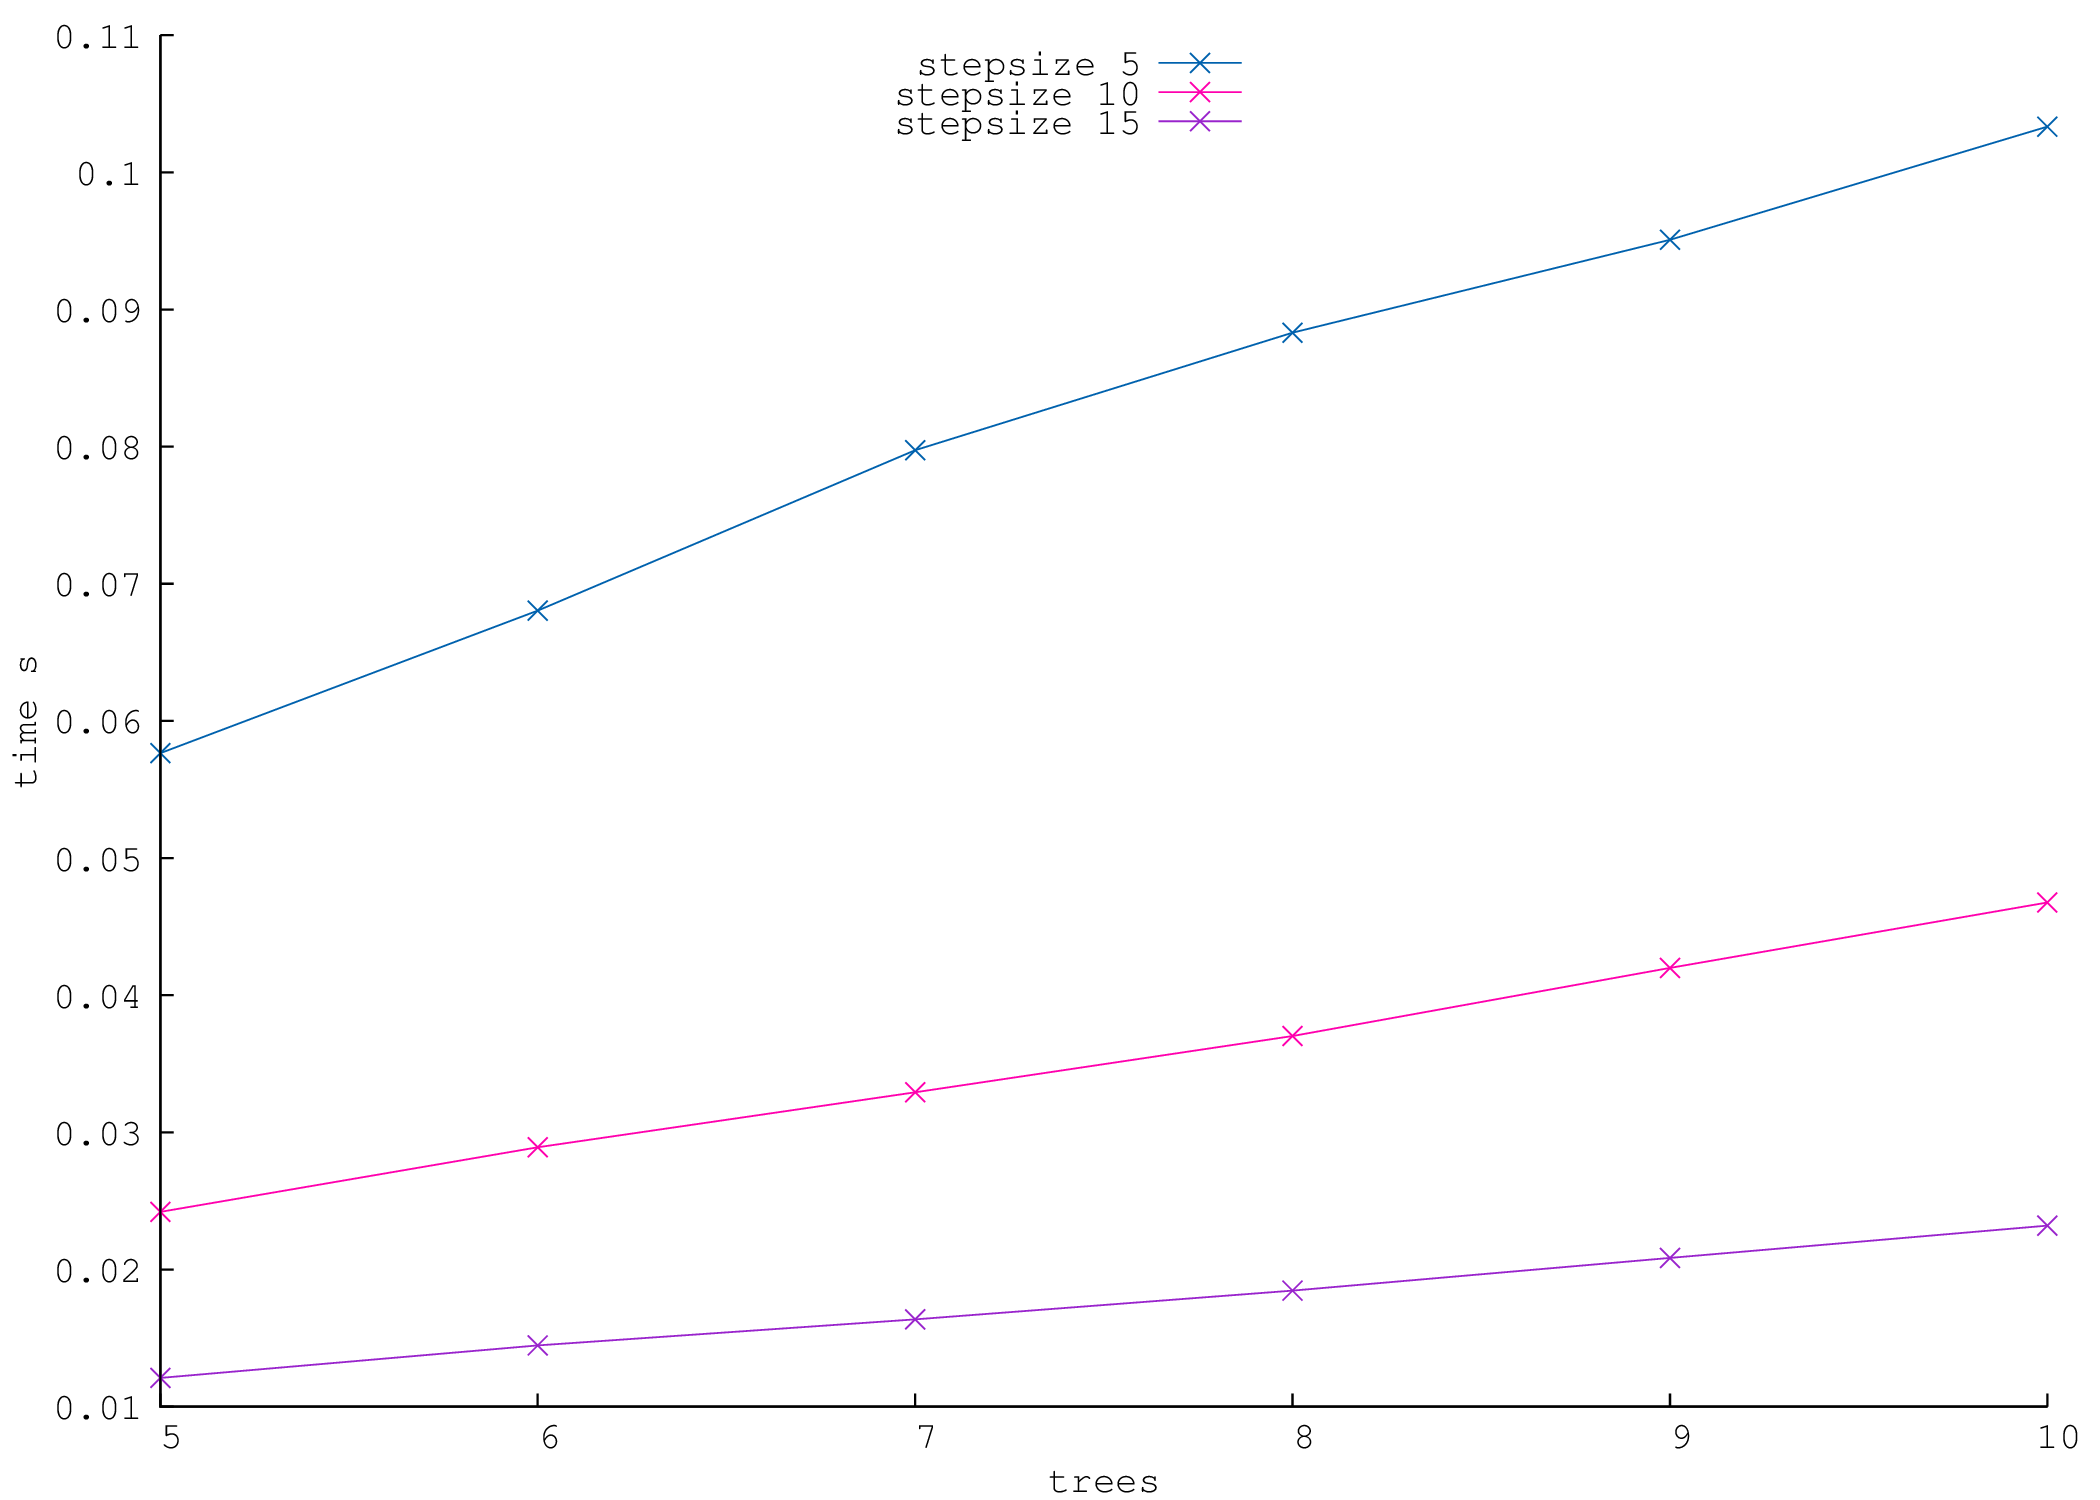
\includegraphics[width=0.8\linewidth]{time.png}
	\caption[Processing time vs number of trees]{\label{fig:time}}  \textbf{average processing time for each image(frame)various densities, stride 5,10,15 in blue,pink,purple respectively }
\end{figure}